\documentclass[12pt]{article}
\usepackage[utf8]{inputenc}
\usepackage{amsmath, amssymb, amsfonts}
\usepackage{geometry}
\usepackage{enumitem}
\usepackage{tikz}
\usepackage{xcolor}
\usepackage{comment}
\geometry{margin=1in}
\setlist[enumerate]{leftmargin=*}

\title{Solutions -- Quiz 1\\ \vspace{10pt}
\large ECON 320 -- Introduction to Mathematical Economics}
\author{Instructor: Muhebullah Karimzada}
\date{September 17, 2025}

\begin{document}
\maketitle

\section*{Q1 Absolute-Value Inequality}
\textbf{Problem. } Solve the inequality
\[
|2x - 5| < 7
\]
and represent the solution set on the real line. Interpret in economic terms if $x$ is quantity and the inequality represents a feasible demand constraint.

\subsection*{Solution}
Recall that for any real $u$ and any $a>0$, $|u|<a \iff -a < u < a$. Let $u=2x-5$ and $a=7$:
\[
-7 < 2x - 5 < 7.
\]
Add $5$ to all three parts:
\[
-2 < 2x < 12.
\]
Divide by $2$:
\[
-1 < x < 6.
\]
Hence, the solution set is the open interval $(-1,\,6)$.

\medskip
\noindent \textbf{Number-line representation.} (Open endpoints at $x=-1$ and $x=6$)
\begin{center}
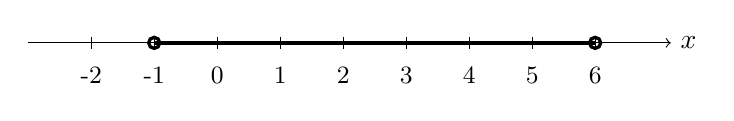
\begin{tikzpicture}[x=0.8cm, y=0.8cm]
  \draw[->] (-3,0) -- (7.2,0) node[right] {$x$};
  \foreach \x in {-2,-1,0,1,2,3,4,5,6}
    \draw (\x,0.1) -- (\x,-0.1) node[below=3pt] {\small \x};
  % open circles
  \draw[very thick] (-1,0) circle (2pt);
  \draw[very thick] (6,0) circle (2pt);
  % interval
  \draw[line width=1.2pt] (-1,0) -- (6,0);
\end{tikzpicture}
\end{center}

\noindent \textbf{Economic interpretation.} If $x$ denotes quantity and the inequality encodes a feasible \emph{demand} region, then all quantities $x\in(-1,6)$ are feasible. Since negative quantities are typically not economically meaningful, one would usually intersect with $x\ge 0$, yielding $x\in[0,6)$ in practical applications.

\bigskip

\section*{Q2.  Feasible Set and Resource Allocation}
\textbf{Problem. } Consider
\[
S = \{ (x,y) \in \mathbb{R}^2 \mid x + y \leq 10, \, x \geq 0, \, y \geq 0 \}.
\]
(a) Sketch $S$. \;\\
(b) If $y=2$, what values of $x$ are admissible? \;\\
(c) Interpret this as a resource allocation problem.

\subsection*{Solution}
(a) The boundary $x+y=10$ has intercepts $(10,0)$ and $(0,10)$. Together with $x\ge 0$ and $y\ge 0$, the feasible set is the filled right triangle in the first quadrant below (and including) the line $x+y=10$.

\begin{center}
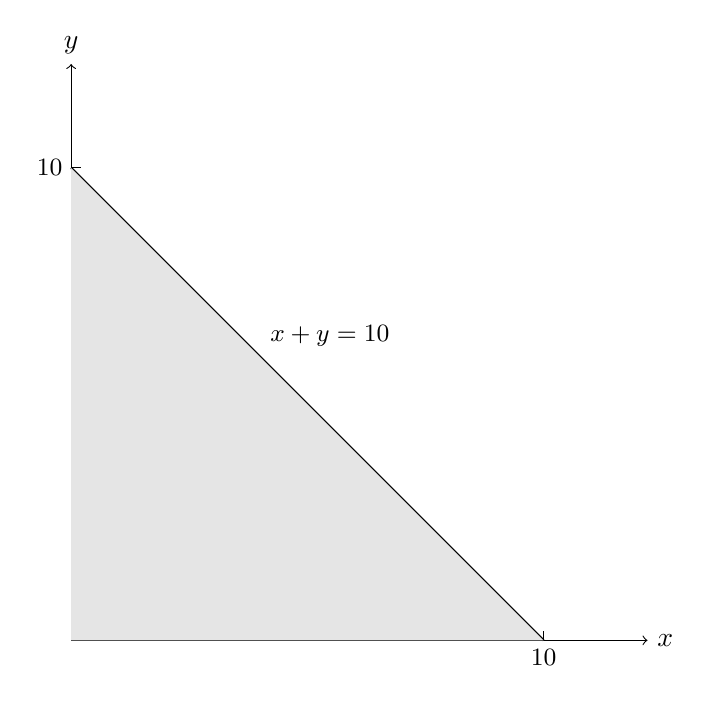
\begin{tikzpicture}[scale=0.6]
  % axes
  \draw[->] (0,0) -- (12.2,0) node[right] {$x$};
  \draw[->] (0,0) -- (0,12.2) node[above] {$y$};
  % boundary line
  \draw[thick] (10,0) -- (0,10) node[pos=0.6, above right] {\small $x+y=10$};
  % shaded feasible region
  \fill[gray!20] (0,0) -- (10,0) -- (0,10) -- cycle;
  % ticks
  \draw (10,0) -- (10,0.2) node[below=3pt] {\small 10};
  \draw (0,10) -- (0.2,10) node[left=3pt] {\small 10};
\end{tikzpicture}
\end{center}

(b) If $y=2$, the constraint $x+y\le 10$ becomes $x+2\le 10$, i.e.\ $x\le 8$. With $x\ge 0$, the admissible set is
\[
0 \le x \le 8.
\]

(c) \textbf{Resource allocation interpretation.} Suppose a planner has $10$ units of a resource to allocate between two nonnegative uses $x$ and $y$. The set $S$ is the budget (or capacity) set. Any point below the line uses fewer than $10$ units; points on the line use exactly $10$ units.

\bigskip
\newpage

\section*{Q3.  Implicit Demand and Total Differentiation}
\textbf{Problem. } Consider the demand relation
\[
Q^d(P,Y) = Y - P^2 = 0,
\]
where $P$ is price and $Y$ is income.
(a) Derive $\dfrac{dP}{dY}$. \;
(b) What does its sign imply about the relationship between income and the equilibrium price?

\subsection*{Solution}
From $Y - P^2 = 0$ we can (for $P\ge 0$) write $P=\sqrt{Y}$, which already suggests $P$ increases with $Y$ for $Y\ge 0$. Using \emph{implicit differentiation}:
\[
\frac{d}{dY}\big(Y - P^2\big) \;=\; 1 - 2P\,\frac{dP}{dY} \;=\; 0
\quad\Longrightarrow\quad
\frac{dP}{dY} \;=\; \frac{1}{2P}.
\]
Equivalently, using $P=\sqrt{Y}$,
\[
\frac{dP}{dY} \;=\; \frac{1}{2\sqrt{Y}}, \qquad (Y>0).
\]

\textbf{Sign and interpretation.} Since $P>0$ at interior solutions, $\dfrac{dP}{dY}>0$: as income rises, the equilibrium price consistent with $Y-P^2=0$ increases. Moreover, $\dfrac{dP}{dY}$ is \emph{diminishing} in $P$ (and in $Y$): the marginal effect of income on price is larger at lower income levels and shrinks as income grows.

\bigskip
\begin{comment}
\section*{Q4. Sign Logic in Comparative Statics}
\textbf{Problem. } Let $F(x,p)=0$ define an equilibrium $x(p)$. Assume $F_x(x,p)<0$ for all relevant $(x,p)$. Prove that the sign of
\[
\frac{dx}{dp} \;=\; -\,\frac{F_p}{F_x}
\]
depends only on the sign of $F_p$. Explain how this allows economists to predict comparative statics without solving explicitly for $x(p)$.

\subsection*{Solution}
\textbf{Step 1: Existence of $x(p)$ and formula for $\dfrac{dx}{dp}$.}
Assume $F$ is continuously differentiable and that at a point $(x_0,p_0)$ we have $F(x_0,p_0)=0$ and $F_x(x_0,p_0)\neq 0$. By the Implicit Function Theorem, there exists a neighborhood of $p_0$ in which a unique continuously differentiable function $x(p)$ satisfies $F\big(x(p),p\big)=0$. Differentiating $F\big(x(p),p\big)\equiv 0$ with respect to $p$:
\[
F_x\,\frac{dx}{dp} + F_p \;=\; 0
\quad\Longrightarrow\quad
\frac{dx}{dp} \;=\; -\,\frac{F_p}{F_x}.
\]

\textbf{Step 2: Sign logic under $F_x<0$.}
If $F_x<0$, then the denominator is negative. Consider two cases for $F_p$:
\begin{itemize}
  \item If $F_p>0$, then $-F_p<0$ and $(-F_p)/F_x = (\text{negative})/(\text{negative})>0$. Hence $\dfrac{dx}{dp}>0$.
  \item If $F_p<0$, then $-F_p>0$ and $(-F_p)/F_x = (\text{positive})/(\text{negative})<0$. Hence $\dfrac{dx}{dp}<0$.
\end{itemize}
Therefore,
\[
\operatorname{sign}\!\left(\frac{dx}{dp}\right) \;=\; \operatorname{sign}\!\big(F_p\big)\qquad\text{whenever }F_x<0.
\]

\textbf{Economic interpretation.} The condition $F_x<0$ means that, holding $p$ fixed, an increase in $x$ \emph{reduces} $F$. Graphically, the $F=0$ locus has a negative (local) slope in the $(x,F)$ direction w.r.t.\ $x$. A parameter change that increases $F$ (i.e.\ $F_p>0$) must then be offset by an increase in $x$ to bring $F$ back to zero, implying $\dfrac{dx}{dp}>0$; analogously for $F_p<0$. 

\textbf{Why this is useful.} Often $F$ encodes equilibrium conditions (e.g., first-order conditions or market-clearing), and $F_x<0$ captures stability/concavity. Then $\operatorname{sign}\big(\dfrac{dx}{dp}\big)$ is determined by the direction the parameter $p$ \emph{pushes} the equilibrium condition ($F_p$), allowing a correct prediction for the effect of $p$ on $x$ \emph{without} explicitly solving for $x(p)$.
\end{comment}
\end{document}
